\documentclass[a4paper,12pt]{report}
\usepackage[utf8]{inputenc}
\usepackage[francais]{babel}
\usepackage{fancyhdr}
\usepackage{graphicx}
\usepackage{tikz}
\usetikzlibrary{calc}
\usepackage{listings}
\usepackage{xcolor}
\definecolor{grey}{rgb}{0.9,0.9,0.9}
\usepackage{titlesec}
\usepackage{verbatim}
\usepackage{listings}
\usepackage{textcomp}
\usepackage{hyperref}
\usepackage{longtable}
\usepackage{colortbl}
\usepackage{amssymb}


\frenchbsetup{StandardLists=true}
\newcommand{\marge}{18mm}
\usepackage[left=\marge,right=\marge,top=\marge,bottom=\marge]{geometry}
\pagestyle{fancy}
\setlength{\headheight}{14pt}
\chead{
  \textbf{Binôme :} Douaille Erwan 
  \hspace{2em}
  \textbf{Groupe :} M2 Info IVI}
\renewcommand{\headrulewidth}{1pt}
\linespread{1}
\setlength{\columnseprule}{0.2pt}
\definecolor{javakeyword}{rgb}{0,0,0.5}
\definecolor{javastring}{rgb}{0,0.5,0}
\definecolor{javacomment}{rgb}{0.5,0.5,0.5}
\lstdefinestyle{Java}{
   language=Java, basicstyle=\footnotesize,       % the size of the fonts that are used for the code
  numbers=left,                   % where to put the line-numbers
  numberstyle=\tiny\color{gray},  % the style that is used for the line-numbers
  stepnumber=1,                   % the step between two line-numbers. If it's 1, each line
                                  % will be numbered
  numbersep=5pt,                  % how far the line-numbers are from the code
  backgroundcolor=\color{white},  % choose the background color. You must add \usepackage{color}
  showspaces=false,               % show spaces adding particular underscores
  showstringspaces=false,         % underline spaces within strings
  showtabs=false,                 % show tabs within strings adding particular underscores
  frame=single,                   % adds a frame around the code
  rulecolor=\color{black},        % if not set, the frame-color may be changed on line-breaks within not-black text (e.g. commens (green here))
  tabsize=2,                      % sets default tabsize to 2 spaces
  captionpos=b,                   % sets the caption-position to bottom
  breaklines=true,                % sets automatic line breaking
  breakatwhitespace=false,        % sets if automatic breaks should only happen at whitespace
  title=\lstname,                 % show the filename of files included with \lstinputlisting;
   stringstyle=\color{javastring},
   keywordstyle=\color{javakeyword}\ttfamily\textbf,
   commentstyle=\color{javacomment}\ttfamily\textit
 }
 

\begin{document}



\makeatletter
\begin{titlepage}
\centering
\vspace{-10em}
{\LARGE \textbf{\textsc{Rapport de Projet RVI}}}\\
\vspace{3em}

\includegraphics[scale=0.6]{image/thalassa.png}\\
\vspace{3em}
{\LARGE \textsc{Projet Thalassa: simulation de plongée sous-marine}}\\

\vspace{8em}
Par\\
\vspace{1em}
{\LARGE \@author}\\

\vspace{2em}



\begin{tikzpicture}[remember picture,overlay]

\node [below left,xshift=-1cm, yshift=4cm] at (current page.south east){
\includegraphics[scale=0.6]{image/ustl1.png}};

\end{tikzpicture}
\end{titlepage}
\makeatother

\sloppy

\setcounter{page}{1} 
\newpage

\section*{Éxécuter le programme}

\begin{lstlisting}[style=Java]
java -jar tp1_Douaille_SMA.jar
\end{lstlisting}

Pour des raison de facilité, il n'y a aucun paramètre à fournir au \textit{.jar}. Une grande partie des fonctionnalitées se règlent via le menu.

\begin{figure}[!ht]
	\center
	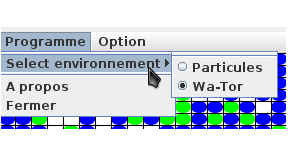
\includegraphics[scale=0.4]{./image/menu2.png}
	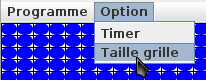
\includegraphics[scale=0.4]{./image/menu1.png}
\end{figure}

\textit{Particules}, \textit{Wa-Tor} et \textit{Ségrégation} sont disponible via ce menu.

\newpage

\section*{Wa-Tor}
\subsection*{Analyse du graphique}

\begin{figure}[!ht]
	\center
	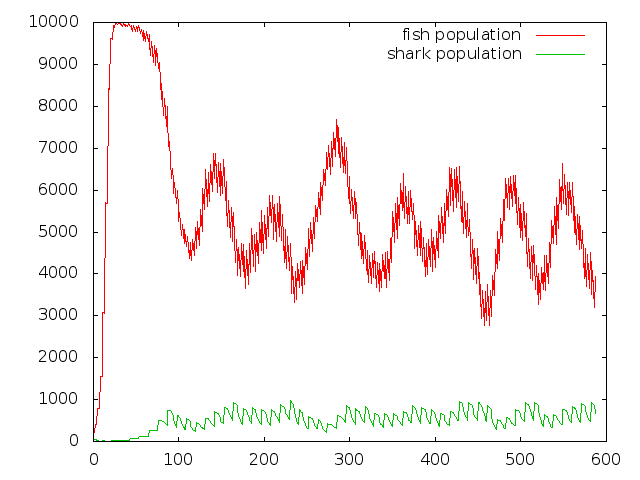
\includegraphics[scale=0.4]{./image/graph.png}
	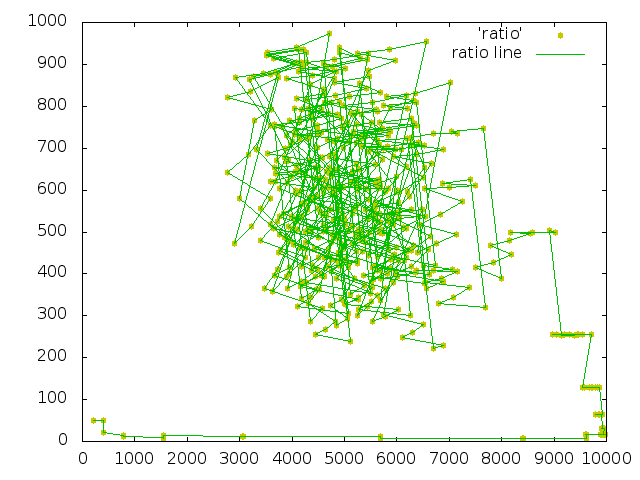
\includegraphics[scale=0.4]{./image/ratio.png}
\end{figure}

Ces deux graphiques sont indépendants.

Sur ces graphiques on observe des \textit{cycles}. Lorsque la population de poisson augmente on observe que quelques secondes plus tard la population de requin augmente également. Le même phénomène est observé lorsque la population de poisson diminue. Moins de poisson donne plus de mort de requin.

En fonction du début de la simulation, l'équilibre des populations reste stable. Il est possible qu'avec des petites taille de tableau, que les requins n'arrivent pas à manger rapidement et donc meurent.

Le ratio montre qu'il éxiste une corrélation entre les cycles et le nombre de poisson divisé par le nombre de requin.
\subsection*{UML et explication de code}

\begin{figure}[!ht]
	\center
	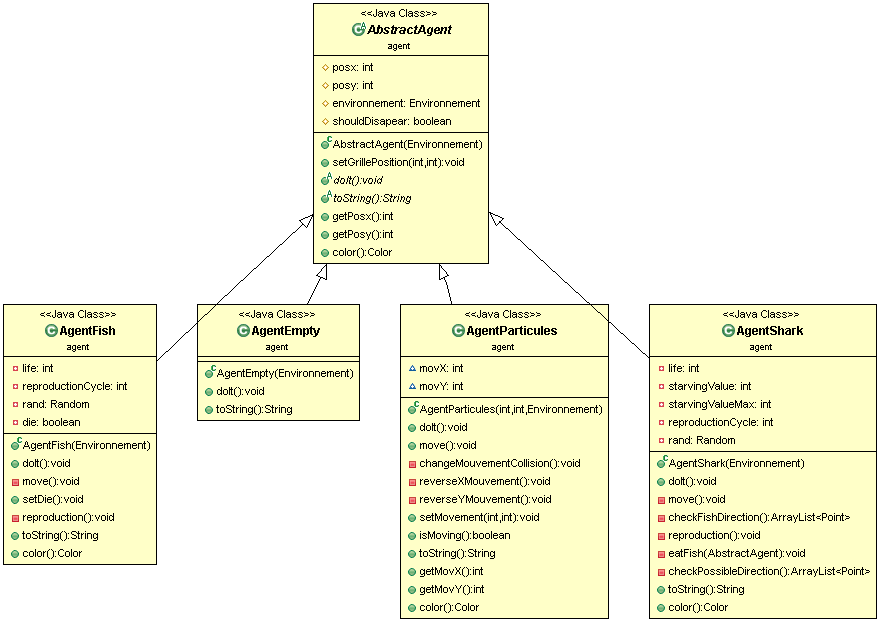
\includegraphics[scale=0.4]{./image/a.png}
	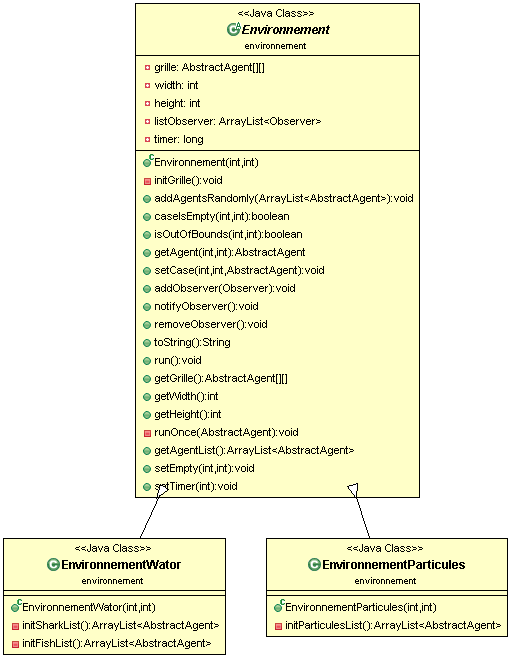
\includegraphics[scale=0.4]{./image/b.png}
\end{figure}


\subsubsection*{Classe agents}

La classe Abstract agent définit des méthodes qui devront être implémenter par les sous agents. AgentEmpty est la représentation d'une case vide.

\textit{AgentShark} et \textit{AgentFish} représentent les agents pour le Wa-Tor et chacun d'eux contient des actions spécifiques à leurs types (manger, reproduction ...).

Les requins et les poissons se déplacent aléatoirement. Si aucun déplacement n'est possible il n'y a pas d'action. Pour les requins, le déplacement est aléatoire mais si des poissons sont présents dans les case adjacentes, un poisson sera choisit aléatoirement. Ce phénomène empêche une mort trop importante des requins dûe à l'aléatoire.

\subsubsection*{Classe Environnements}

\textit{Environnement} définit le coeur du système. La boucle qui va itérer sur le tableau d'agents et leurs faire éxécuter leurs actions. Environnement contient également le code nécessaire pour notifier les observers d'une mise à jour (\textit{cf MVC}).

\textit{EnvironnementWator} définie les agents fish et shark a ajouter dans la superclass.

\textit{EnvironnementParticules} définie les agents particules a ajouter dans la superclass.

\subsubsection*{MVC}

L'interface graphique est réalisée en MVC. Les réglages des environnements est disponible via le menu.

La librairie \textit{JFreeChart} a été utilisée pour faire les graphiques (facile d'utilisation et rapide). Le prochain TP je ferais les graphes avec GNU Plot avec une sortie des valeurs dans des fichiers de log.
\newpage


\section*{Ségrégation}

La ségrégation consiste à mettre sur une grille deux population avec un seuil de satisfaction. Si l'agent à une satisfaction supérieur au seuil alors il ne se déplace pas. La satisfaction est calculé en comptant le nombre de populations opposées adjacents divisé par le nombre total d'agents adjacents.

\subsection*{Analyse du graphique}

Dans la partie \textit{ségrégation} notre objectif a été de déterminer quels sont les seuils à fixer pour obtenir une stabilisation de la population.

Nous avons définit dans le code que 40\% de la surface disponible serait des rouges et 40\% des verts, pour remplir au maximum la surface tout en laissant un minimum de cases vides pour permettre le déplacement des agents.

Voici ce que nous obtenons comme résultats:
\begin{center}
\begin{table}[h]
\begin{center}
\begin{tabular}{|l|l|l|ll}
\cline{1-3}
0-100\% satisfaction & Rouge & Vert &  &  \\ \cline{1-3}
0 & 0 & 0 &  &  \\ \cline{1-3}
1 & 0 & 0 &  &  \\ \cline{1-3}
2 & 0 & 0 &  &  \\ \cline{1-3}
3 & 0 & 0 &  &  \\ \cline{1-3}
4 & 0 & 0 &  &  \\ \cline{1-3}
5 & 0 & 0 &  &  \\ \cline{1-3}
6 & 0 & 0 &  &  \\ \cline{1-3}
7 & 20 & 26 &  &  \\ \cline{1-3}
8 & 34 & 30 &  &  \\ \cline{1-3}
9 & 262 & 150 &  &  \\ \cline{1-3}
\end{tabular}
\end{center}
\caption{Table des pourcentages}
\label{my-label}
\end{table}
\end{center}

\begin{figure}[!ht]
	\center
	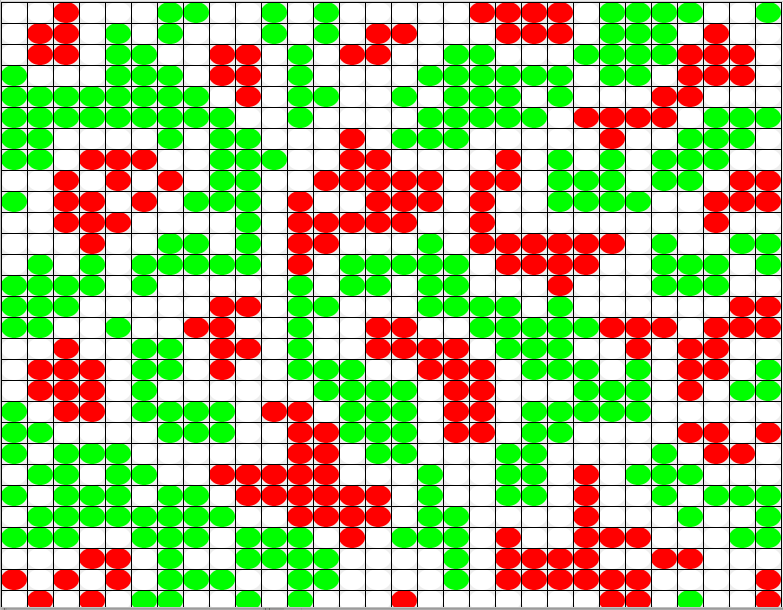
\includegraphics[scale=0.4]{./image/segregation.png}
\end{figure}

Le taux de satisfaction sur cet exemple était fixé à 70\%. On observe içi que tout le monde a "\textit{trouvé ça place}", tout le monde est satisfait.

Avec plusieurs tests on a remarqué qu'en influent sur la population (nombres d'agents) et sur la satisfaction, le graphique se stabilise plus ou moins vite.

Avec 80\% de satisfaction on observe des groupes persistents et des agents qui se déplacent sans trouver une satisfaction satisfaisante. Testé sur quelques minutes à partir d'environ 80\% avec 80\% de places occupées par les agents, la population ne se stabilise pas.

Lorsqu'une taille de grille importante est définit la stabilisation est compliquée. Sur une taille de grille de \textit{100$\times$100} avec 80\% de population et une satisfaction de 70\%, au bout de quelques minutes, aucune stabilisation n'a été constaté, même si des regroupements de populations apparaîsent.

\subsection*{Explication de code}

Comme toute la base était présente pour la ségrégation, il a été nécessaire d'ajouter un \textit{AgentSegregation} et une classe \textit{EnvironnementSegregation} (initialise l'environnement).

Concernant les graphiques, pour plus de simplicité des exporters CSV ont été créés. Les fichiers \textit{.plot} sont pr\^ets à être utilisés.

Ils peuvent être lancés via la commande \textit{gnuplot}. Voici un exemple:

\begin{lstlisting}[style=Java]
gnuplot plotRatio.plot
\end{lstlisting}

\newpage

\section*{Pacman}

Pour le jeu du pacman le but est de placer sur une grille un pacman et des fantômes qui poursuivent pacman. Pour que les fantômes trouvent le chemin le plus rapide nous avons utilisé l'algorithme de Dijkstra.

Voici un apercu du résultat:

\begin{figure}[!ht]
	\center
	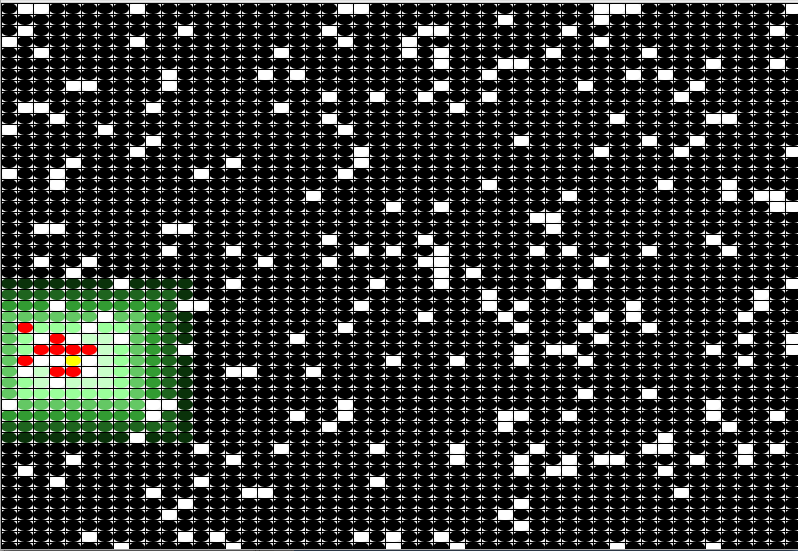
\includegraphics[scale=0.4]{./image/pacman.png}
\end{figure}

Le dégradé de vert sert à indiquer les valeurs sur les cases les plus proches.
Mes agents se déplacent sur les 8 cases adjacentes et non sur 4. Pour faire sur 4 cases il faut rajouter quelques conditions.

\subsection*{Explication de code}

Voici l'algorithme que j'ai utilisé pour créer le disjktra.

\begin{lstlisting}[style=Java]
	private void dijkstraPowa(int x, int y) {	
		for (int i = 0; i < this.width; i++) 
			for (int j = -i; j <= i; j++)
				for (int k = -i; k <= i; k++)
					if (!this.isOutOfBounds(x+j, y+k)) 
						this.setDijkstraTo(x+j, y+k, i);
	}					

	private void setDijkstraTo(int i, int j, int cpt) {
		AbstractAgent agent = this.getAgent(i, j);
		if (agent.getClass().equals(AgentEmptyWithId.class)) {
			AgentEmptyWithId agentID = (AgentEmptyWithId)agent;
			if (agentID.getValue()==0 ) 
				agentID.setValue(cpt);
		}		
	}
\end{lstlisting}

Le principe est je pars de la position de pacman, j'incrémente les cases adjacentes en regardant la valeur minimale des cases adjacentes à celle que je calcule et j'ajoute 1.

Voici une liste des classes que j'ai ajouté:

\textit{AgentGhost} définit le comportement des agents fantômes.

\textit{AgentPacman} définie le comportement de Pacman.

\textit{EnvironnementPacman} surcharge de la classe Environnement. Le calcul de \textit{Dijskstra} est également présent dans cette classe.

\end{document}